\subsection{Proposed abstractions}
As expected for a problem with such a significance, various abstractions have been proposed in order to support the concept of Service-Centric networking.
Deciding the right abstractions premises first the detailed understanding of where a problem resides, and then the genuine intuition for conceiving the simple yet powerful generalizations that better conform with the current and future needs.
Those abstractions should be transparent enough for legacy ports and hot swapping with the prevalent systems, in the meantime powerful to break ground for future advancements.

We appraise the Serval abstractions of \emph{Service Names} and \emph{Flow Identifiers} for being a great solution on the overloading of identifiers within and across the present TCP/IP stack.
Also, for the tight fit of those abstractions in the separation of data and control plane.
Finally, it is remarkable how the adoption of those abstractions requires minimal if no modifications at all in the infrastructure that powers networks today.



\subsubsection{Service Names}
The main idea behind Service-Centric Networking is that nowadays network users request services by their names and are completely agnostic of the underlying procedures.
Hereby an abstraction is needed for identifying a service, resolving and of course effectively routing a request to an instance of that service, according to specific rules.
For that reason Serval introduces service names, or \emph{serviceIDs}.

ServiceIDs are large (256 bit long) strings, that correspond to a service, or a group of services.
Part of Serval packets as a Service Access Extension header in the synchronization process (SYN and SYN-ACK flags in ECCP state machine figure \ref{fig:EECP_sm}), serviceIDs assist in resolution, late binding and service-level routing.
Furthermore they are used as persistent, global identifiers for easier handling of replicated services, and new services quick registration.

What is unique about Serval's abstraction of service identifiers is that since they are managed by the SAL, they are positioned below the transport layer.
Jointly with Serval active sockets, the abstraction of service names obscures host identifiers (IP and Port) from the application layer, but stills offers powerful, familiar APIs\nomenclature{API}{Application Programming Interface} to networked application developers.

Notably, likewise to IP hierarchical notation, serviceIDs can well support a hierarchical address assigning scheme.
In other words, serviceID blocks can be allocated to service providers to assign to their own applications, in a long-prefix matching settlement.
We are discussing extensively hierarchical resolution later on section~\ref{sec:hierresol}.

To sum up, in an elegant way serviceIDs promote services to the principal entities in the network, by giving applications intermediate access to the service control plane.
And they manage to do so while hiding unneeded abstractions, such as the $<IP, port>$ tuple.



\subsubsection{End-host flow identifiers}
The other problem Serval is intending to counteract, is the limitations of PF\_INET sockets' tight binding to the stack.
Since the one responsible for demultiplexing incoming packets is the transport layer, and does so based on identifiers confined to local and remote interfaces, modifying any of those identifiers breaks the connection.
Then is appointed to the protocol to take action in restoring the communication channel.
This issue causes diminished connectivity mutability, forces the overloading of the five tuple $<remote IP, remote port, local IP, local port, protocol>$ across the network stack, and requires the re-implementation of failover functionality by individual protocols.

Serval, and specifically the Service Access Layer, detaches the process of local demultiplexing and provides to the upper layers a single identifier: the \emph{flowID}.
Flows, a notion used before to describe "virtual" network streams, find place in the SAL as the abstraction of socket numbers.
They resemble, in a way, a direct pointer to the local and remote sockets, no matter in which interface, IP address or port they are connected.

\begin{figure}
\centering
\phantomsection
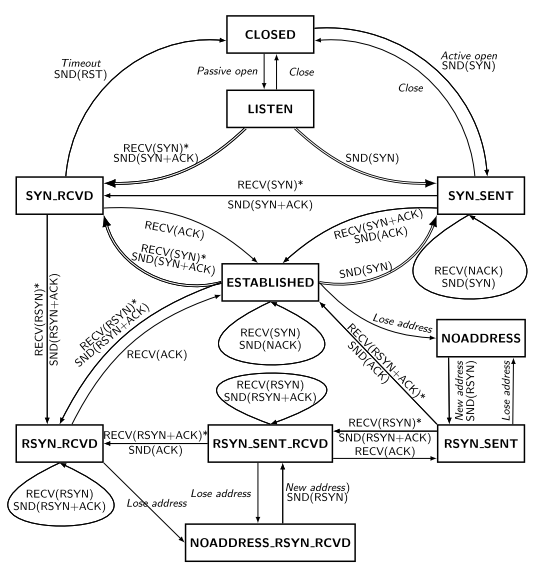
\includegraphics[scale=0.6]{figures/ECCP_sm}
\caption[The ECCP state machine]{The ECCP \cite{Arye2012} state machine.}
\label{fig:EECP_sm}
\end{figure}

This gives the freedom to applications --or even virtual machines-- establish multiple flows, possibly in different interfaces, push and receive traffic to any of them (or a combination of them, increasing bandwidth), without implementing any additional functionality in the protocol residing in the transport layer, or the application.
Everything is settled by the SAL, and a provably correct end-host signalling protocol (figure \ref{fig:EECP_sm}).

When it comes to implementation, flowIDs are 32bit unsigned integers and are end-host specific.
They are created during the synchronization of a new connection and are stored in SAL's flow table, serving as rules for demultiplexing incoming packets to the appropriate sockets.
Source and destination flowIDs are also part of the Serval header in every packet, sitting in the first 64 bits following the IP header.
FlowIDs are persistent, no matter the modifications of any of the values of the five tuple.
Furthermore SAL might assign multiple flows in the same socket, and change them dynamically during its lifetime, in order to ensure maximum bandwidth and continuous connectivity.